\documentclass{scrartcl}			% defines the kind of document you want to produce

% Include different packages:
\usepackage[utf8]{inputenc}
\usepackage[T1]{fontenc}
\usepackage{lmodern}
\usepackage[english]{babel}
\usepackage{amsmath}
\usepackage{float}
\usepackage{graphicx}           	% include graphics
\usepackage{caption}
\usepackage{subcaption}
\usepackage{hyperref}
\usepackage{listings}
\usepackage{fancyvrb}

\title{Neuroprothetik Exercise 4 \\\textsl{}
	Hodgkin \& Huxley Model}

\author{Aleksandra Teska}
\date{7. June 2018}


\begin{document} 					% Document begins here

\maketitle
\section{Time constants and steady state values}		% start a new section
In first exercise we derive the rate equations for all $\alpha_{x}$, $\beta_{x}$, time constant ${\tau_x}$ and steady state value $x_{\infty}$ for $x\in\{m, n, h\}$. The gating ODE was define as:
\begin{align}
\frac{dx}{dt} = \frac{1}{\tau_x} (x_{infty} - x)
\end{align}			

Plots of $tau_x$ and $x_{\infty}$ against the voltage $V \in [-100 mV, 100 mV]$ at temperature of 6.3$^{\circ}$C and 28 $^{\circ}$C were plotted in section 3.1 \\


Gating variables are responsible for activation and inactivation of ion channels. The gating variables \textit{m} and \textit{h} are a part of sodium ionic current equation, their dependency on voltage can be seen in plot \ref{fig1_2}. On the plot we can notice different behavior of each gating variables. \textit{h} responsible for inactivation of the ion channel is open at resting potential and it closes after depolarization of the cell. The other gating variable behave in the opposite way. Additionally, plots prove that the behavior of gating variables is independent of temperature.\\

Time constants define the speed with which voltage value is approaching the target value. On the plot \ref{fig1_1} we can see that they depend on voltage and temperature. Time constants is around 10 times bigger in higher temperature of 28$^{\circ}$C.


\section{Hodgkin \& Huxley Neuron Model}		% start a new sectio
Main goal of this exercise was an implementation of Hodgkin \& Huxley Neuron Model. It is consistent of two parts - calculation of ionic currents and gating ODEs solved with use of exponential-euler solver.

\subsection{Experiments}
For experimental part of the exercise, the model was run for 100 ms (${\Delta t = 0.01 ms}$) with the following settings:
\begin{enumerate}
	\item At 6.3$^{\circ}$C induce a stair of five 5 ms long rectangular current pulses with a gap of
	10 ms and the amplitudes 1 $\mu A/cm^2$, 2 $\mu A/cm^2$, 3 $\mu A/cm^2$, 4 $\mu A/cm^2$, 5 $\mu A/cm^2$
	\item At 28$^{\circ}$C induce a stair of five 5 ms long rectangular current pulses with a gap of
	10 ms and the amplitudes 2 $\mu A/cm^2$ , 4 $\mu A/cm^2$, 8 $\mu A/cm^2$, 16 $\mu A/cm^2$, 32 $\mu A/cm^2$
\end{enumerate}
The plots of the input density currents can be found in section 3.2\\

The following Plots of the results from the two experiments were created:
\begin{enumerate}
	\item Plot the membrane potential over time.
	\item Plot the gating constants m, n, h over time
	\item Plot the current densities $i_{Na}$ , $i_K$ over time.
	\item Plot the current densities $i_{Na}$ , $i_K$ , $i_L$ , over the membrane potential (phase plot).
\end{enumerate}

Plots can be found in section 3.3.

\subsection{Analysis of the Results}

\begin{enumerate}
\item \textbf{Comparison between the results at 6.3$^{\circ}$C and 28$^{\circ}$C:\\}

At temperature of 28$^{\circ}$C gating variables do not change their steady state values. We can notice a change in time constant. In higher temperature its value increases around 10 times. Due to the different time constant values the after stimulation changes are occurring faster - higher temperature means faster processes. Consecutive action potentials in higher temperature have decreasing amplitude - it can be seen in gating variables, ionic currents and finally membrane potential. Phase plots have different trajectories, in case of lower temperature the shape is almost preserved in between spikes.


\item  \textbf{How is an action potential generated and what is the role of the different currents and gating variables:\\}

Action potential happens when the membrane potential gets increased above certain threshold, with external stimulation. That leads to the opening of sodium ion channels (in HH Model opened by the fast gating variable \textit{m}) and causes an inflow of positive sodium ions current into the cell. This inflow causes faster depolarization of the membrane and opening of potassium ion channels (gating variable \textit{n}), that is followed by the outflow of sodium current from the cell.\\ At the same time, gating variable \textit{h} starts to deactivate the sodium channels, which leads to repolarization. Hyperpolarization occurring at the end of action potential happens due to slow closing of the potassium channels (\textit{n} gating variable).

\item \textbf{Explain why consecutive action potentials decrease in amplitude (at 28$^{\circ}$C):\\}

According to the equations of Hodgkin \& Huxley Model - the amplitude of the action potential depends on the ionic current. The ionic current depends on the gating variables \textit{m}, \textit{n} and \textit{h}. Due to the higher temperatures the occurring changes are happening faster. If we take a look at the figure \ref{fig5} we can notice that the gating variables do not decrease back to their original state and afterwards their next change occurs to the lower level.\\

For example in case of m gating variable in original temperature of 6.3$^{\circ}$C it is changing in between 0 and 1, while for higher temperature with each action potential the highest point is lower(going to 0.8 instead of 1). Less open channels, means smaller ionic current density, which means smaller amplitude of an action potential.


\item \textbf{How can you interpret the phase plot.\\}How can you interpret the phase plot.\\

On phase plot we can see the range in which both current densities of ion channels and membrane potential are working. We can notice the dependency of the current densities on the voltage. The shape of an action potential is preserved in case of experimental temperature of 6.3$^{\circ}$C. The action potentials with decreased amplitude, that are happening in higher temperature can be noticed as smaller trajectories.


\item \textbf{Differences between the LIF and the HH model:\\}

LIF model are effective when dealing with question of neuronal processing, it is a great model when we do not have a lot of data or computational power for a more complex model(big ensemble of neurons). But LIF are very 
limited models, it does not take into consideration the biophysical behavior of the cell.\\

Depending on the level of details that is needed, we have to decide which model to use. For analysis of any biophysical properties or more detailed behavior of the cell, we have to use HH model. If we only want to analyze spiking behavior or use neuron as information processing units the LIF model should be enough and giving an additional benefit of saved computational power. 
\end{enumerate}

\newpage
\section{Plots - Solution}
\subsection{Plots of time constants and steady state values}
\begin{figure}[hbpt!]					%start figure-environment
	\begin{flushleft}
		\hspace*{-0.1in}
		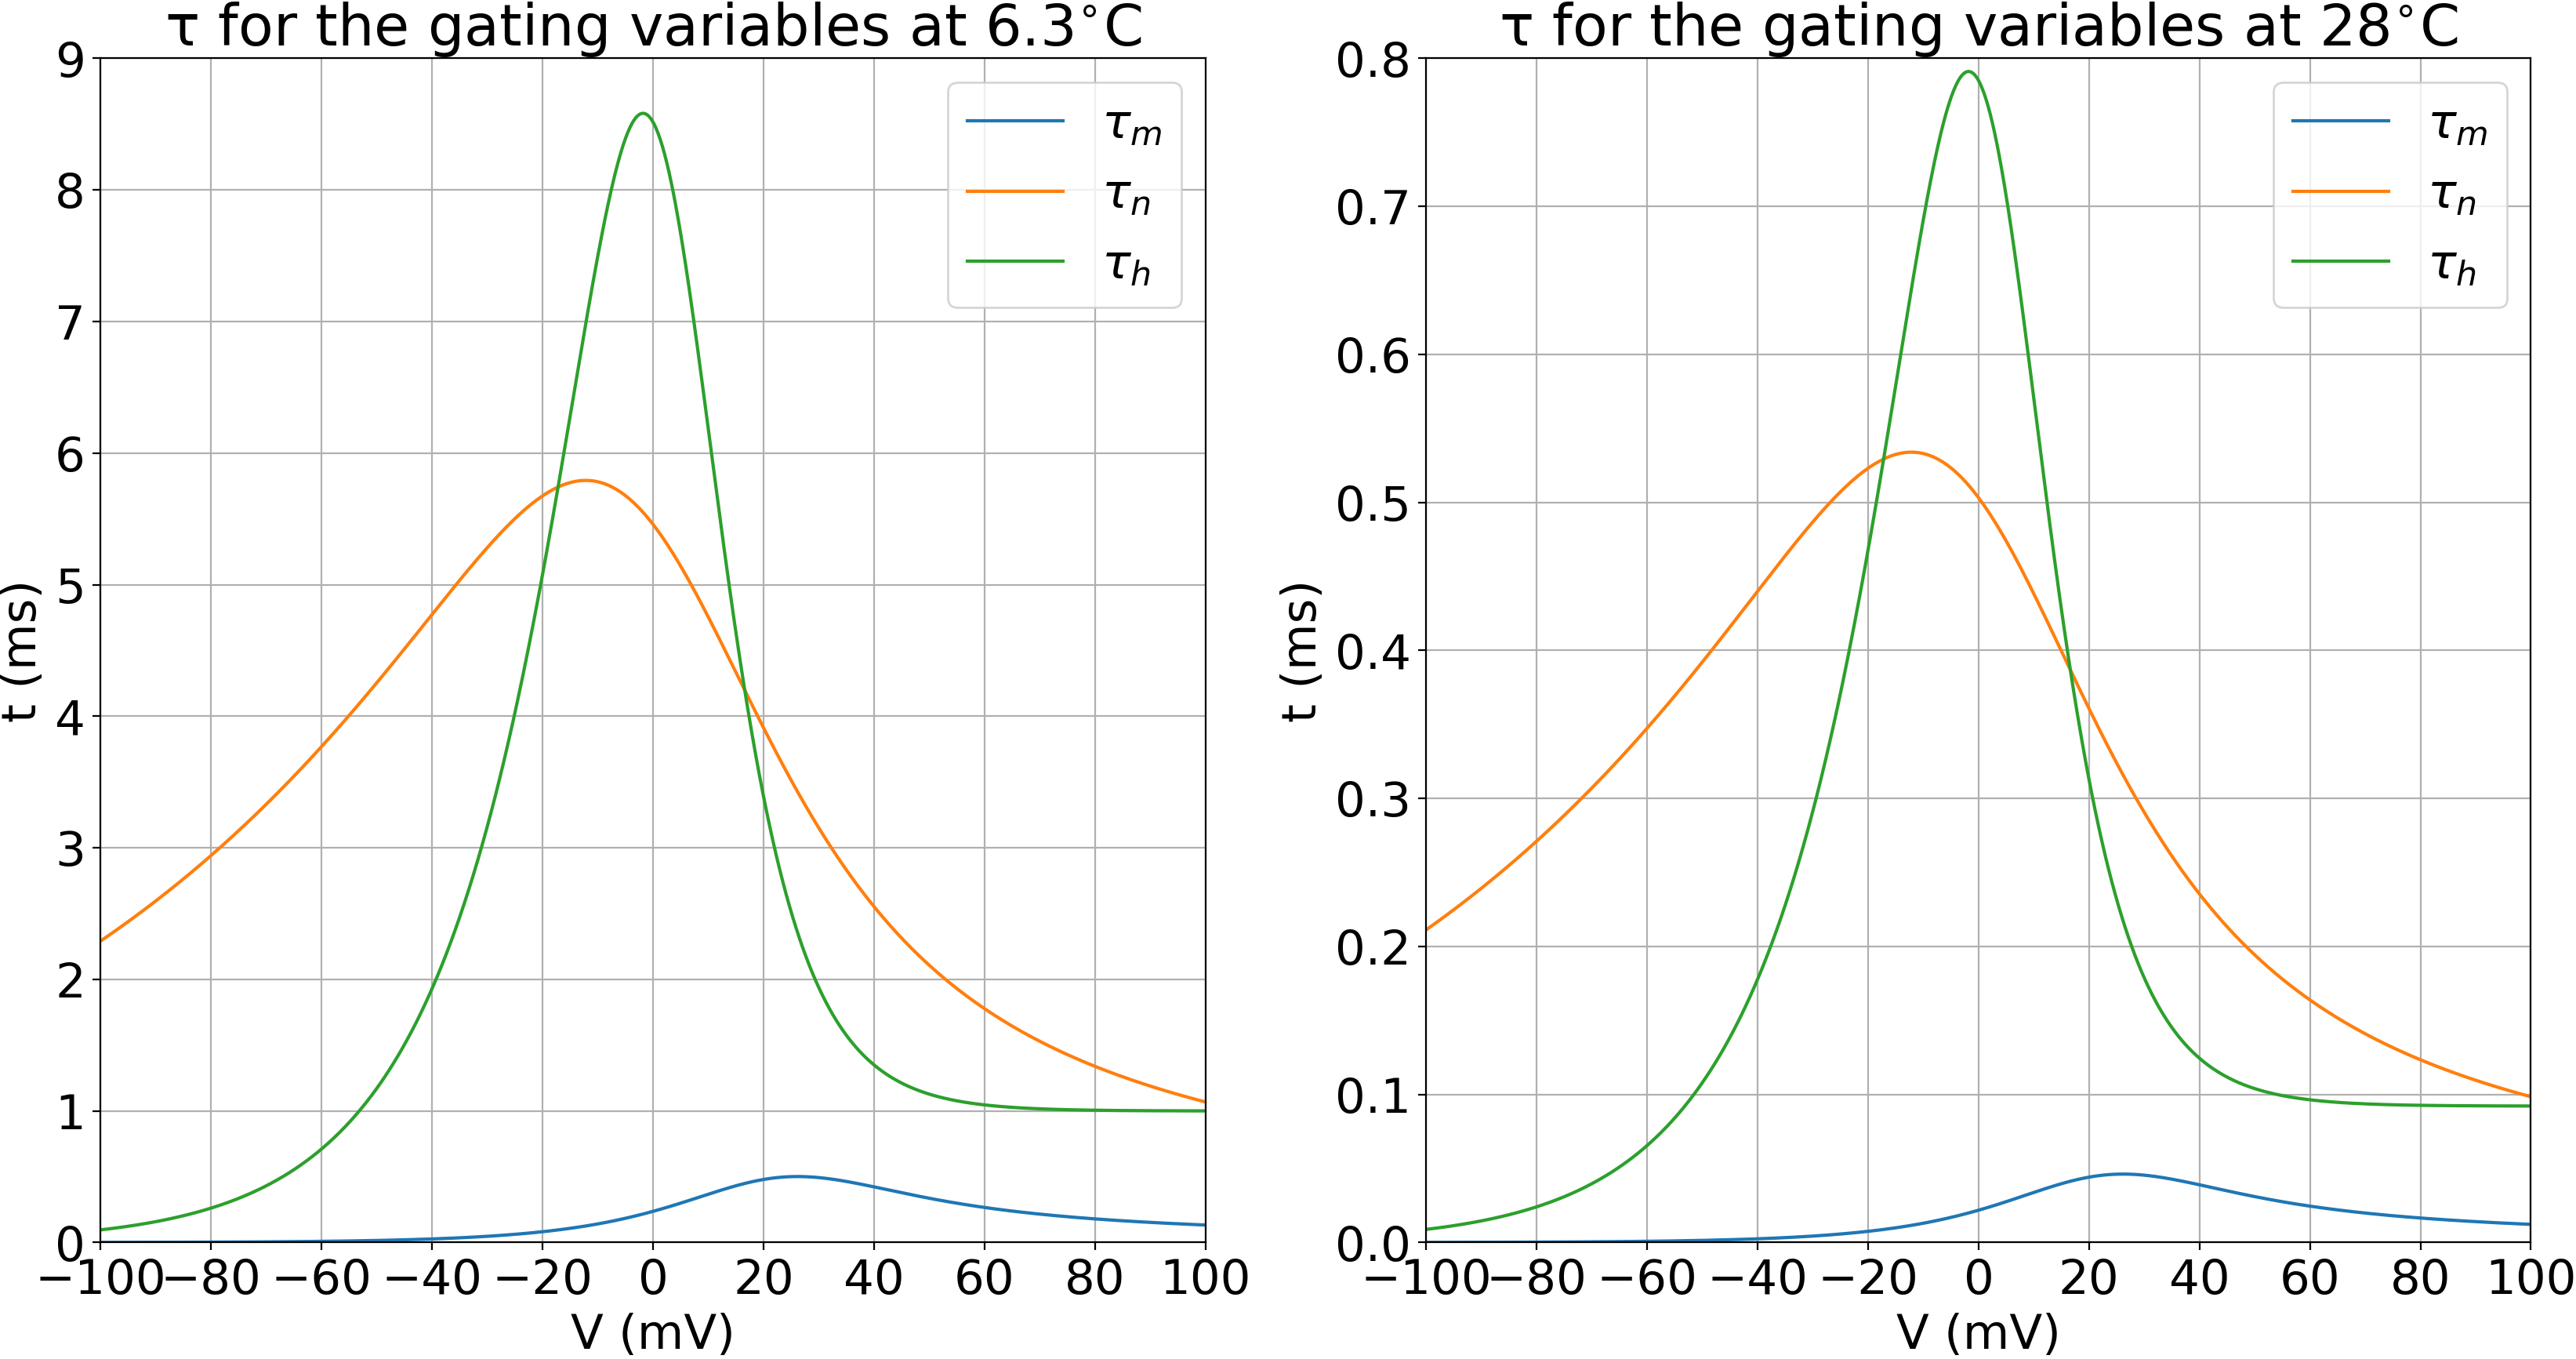
\includegraphics[scale=0.353]{1_1.png}
		\captionsetup{width=\linewidth}  %choose the with of the caption
		\caption{Time constant $\tau$ for the gating variables m, n and h for 6.3$^{\circ}$C and 28$^{\circ}$C.}		
		\label{fig1_1} %choose a label, see subsection references
	\end{flushleft}
\end{figure}

\begin{figure}[hbpt!]					%start figure-environment
	 \begin{flushleft}
		\hspace*{-0.1in}
		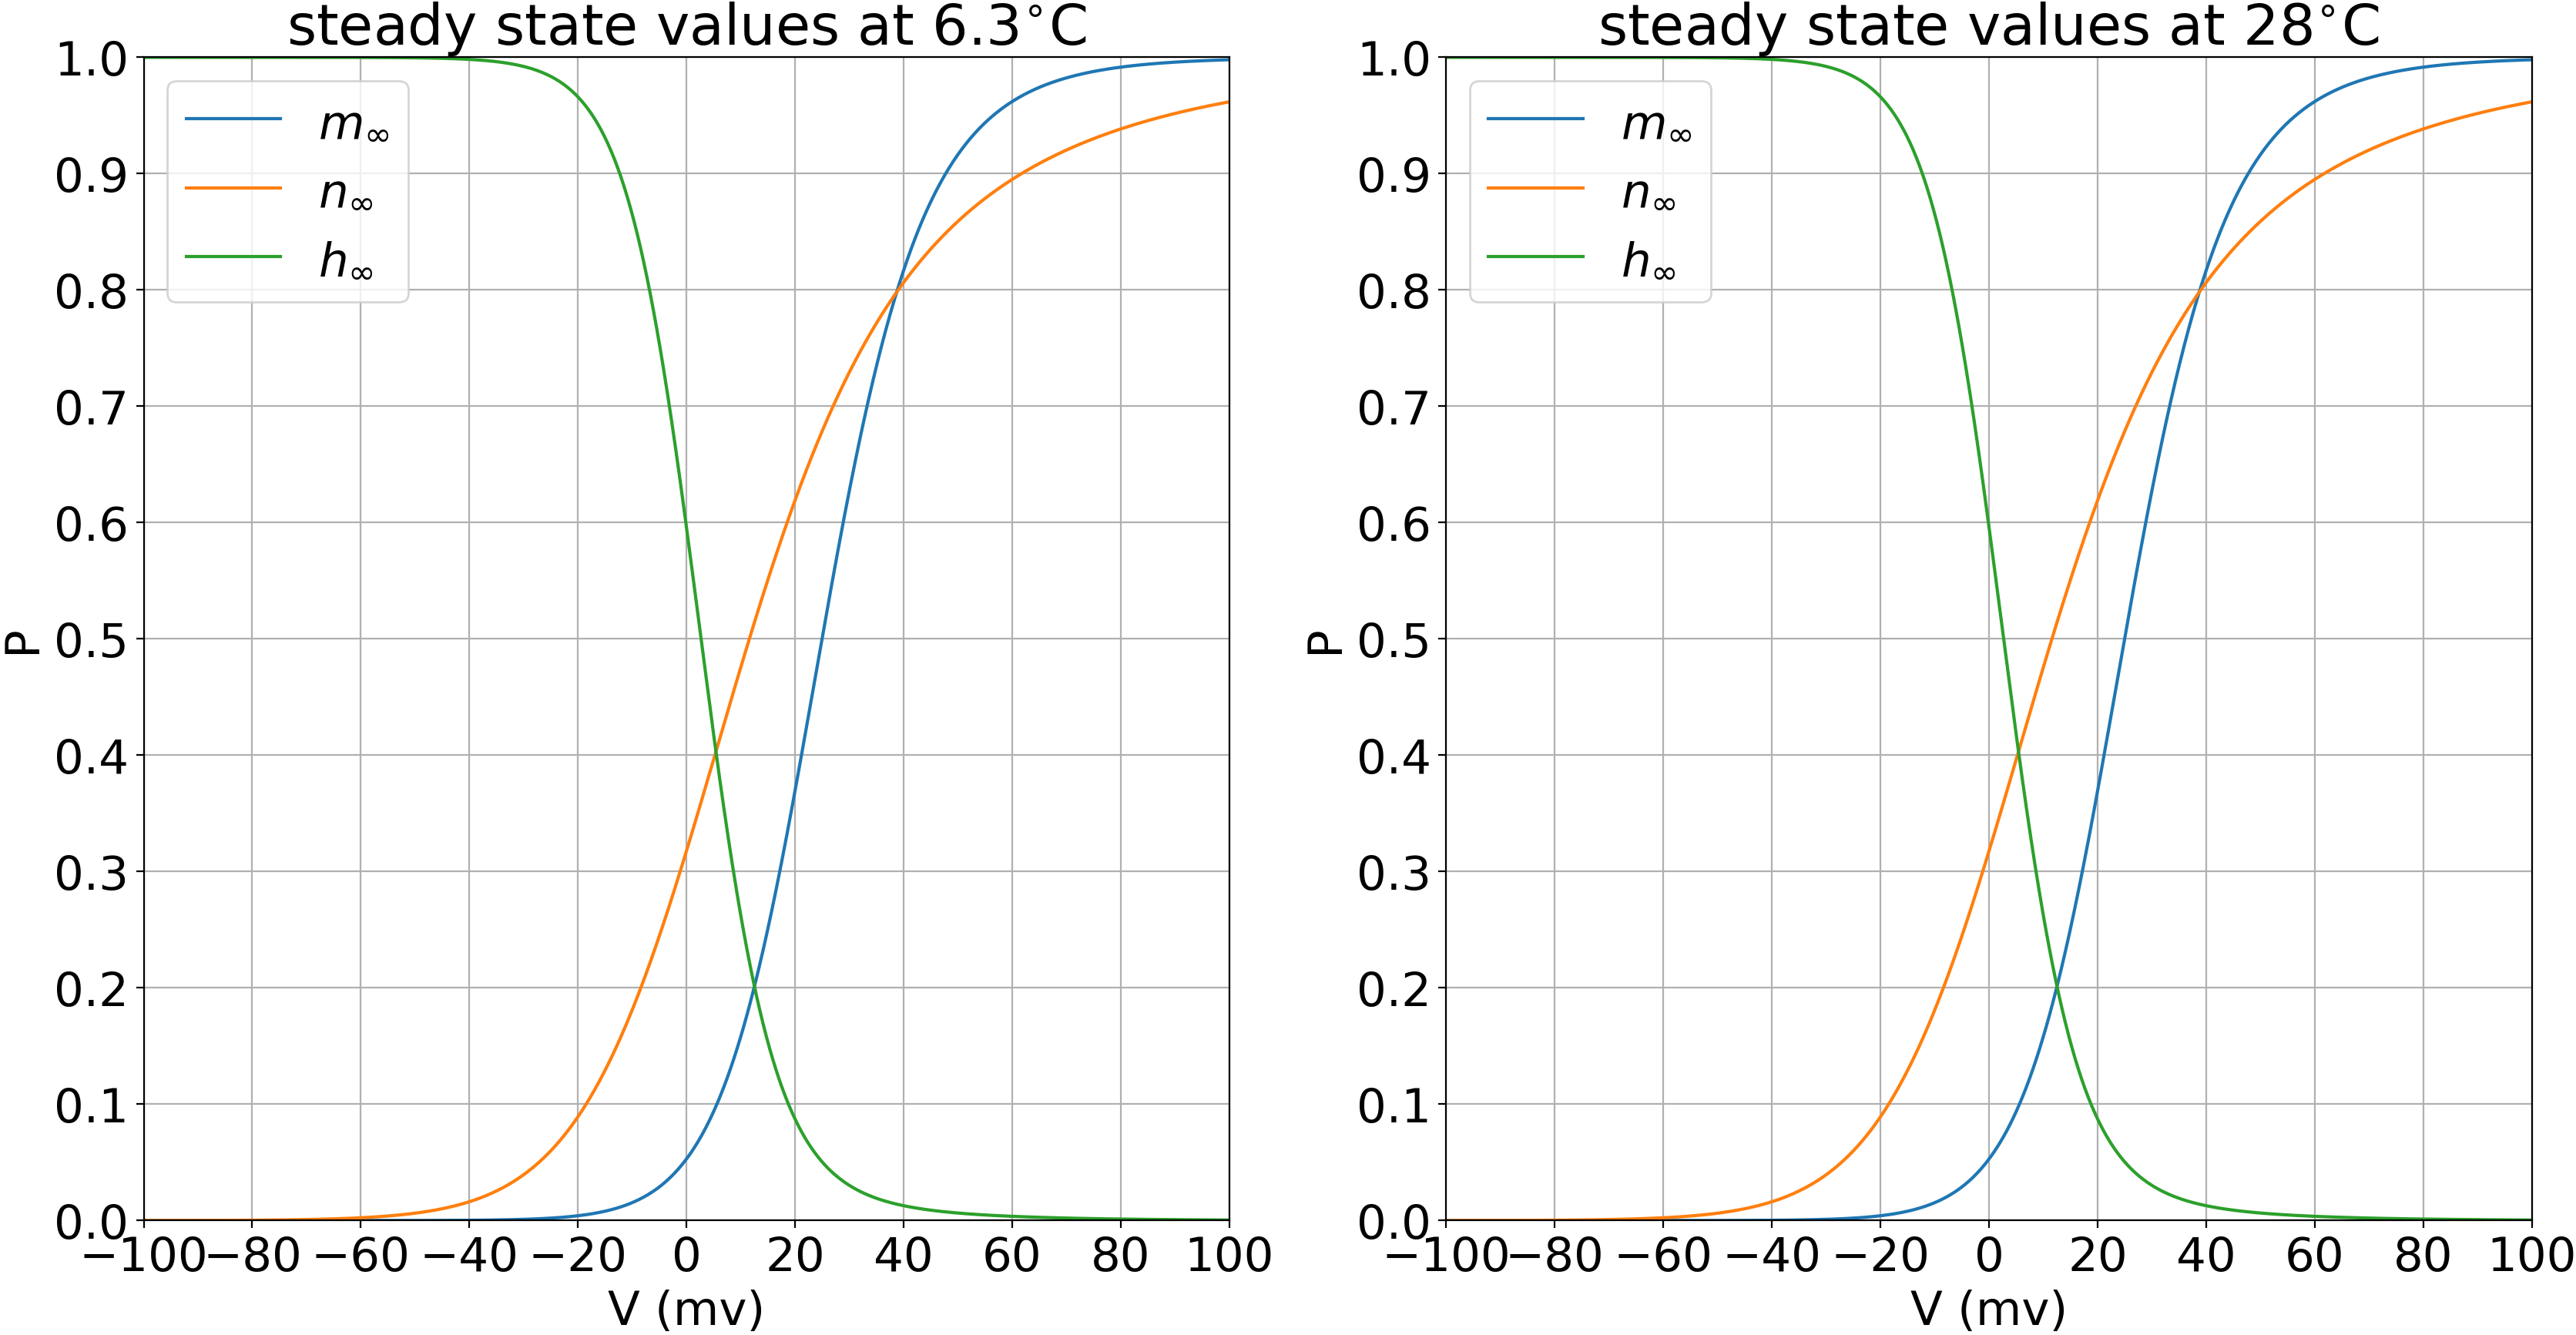
\includegraphics[scale=0.353]{1_2.png}
		\captionsetup{width=\linewidth}  %choose the with of the caption
		\caption{Steady state value $x_{\infty}$ for the gating variables m, n and h for 6.3$^{\circ}$C and 28$^{\circ}$C.}
		\label{fig1_2} %choose a label, see subsection references
	\end{flushleft}
\end{figure}


\newpage
\subsection{Plots of the input current densities}

\begin{figure}[hbpt!]					%start figure-environment
	\begin{flushleft}
		\hspace*{-0.1in}
		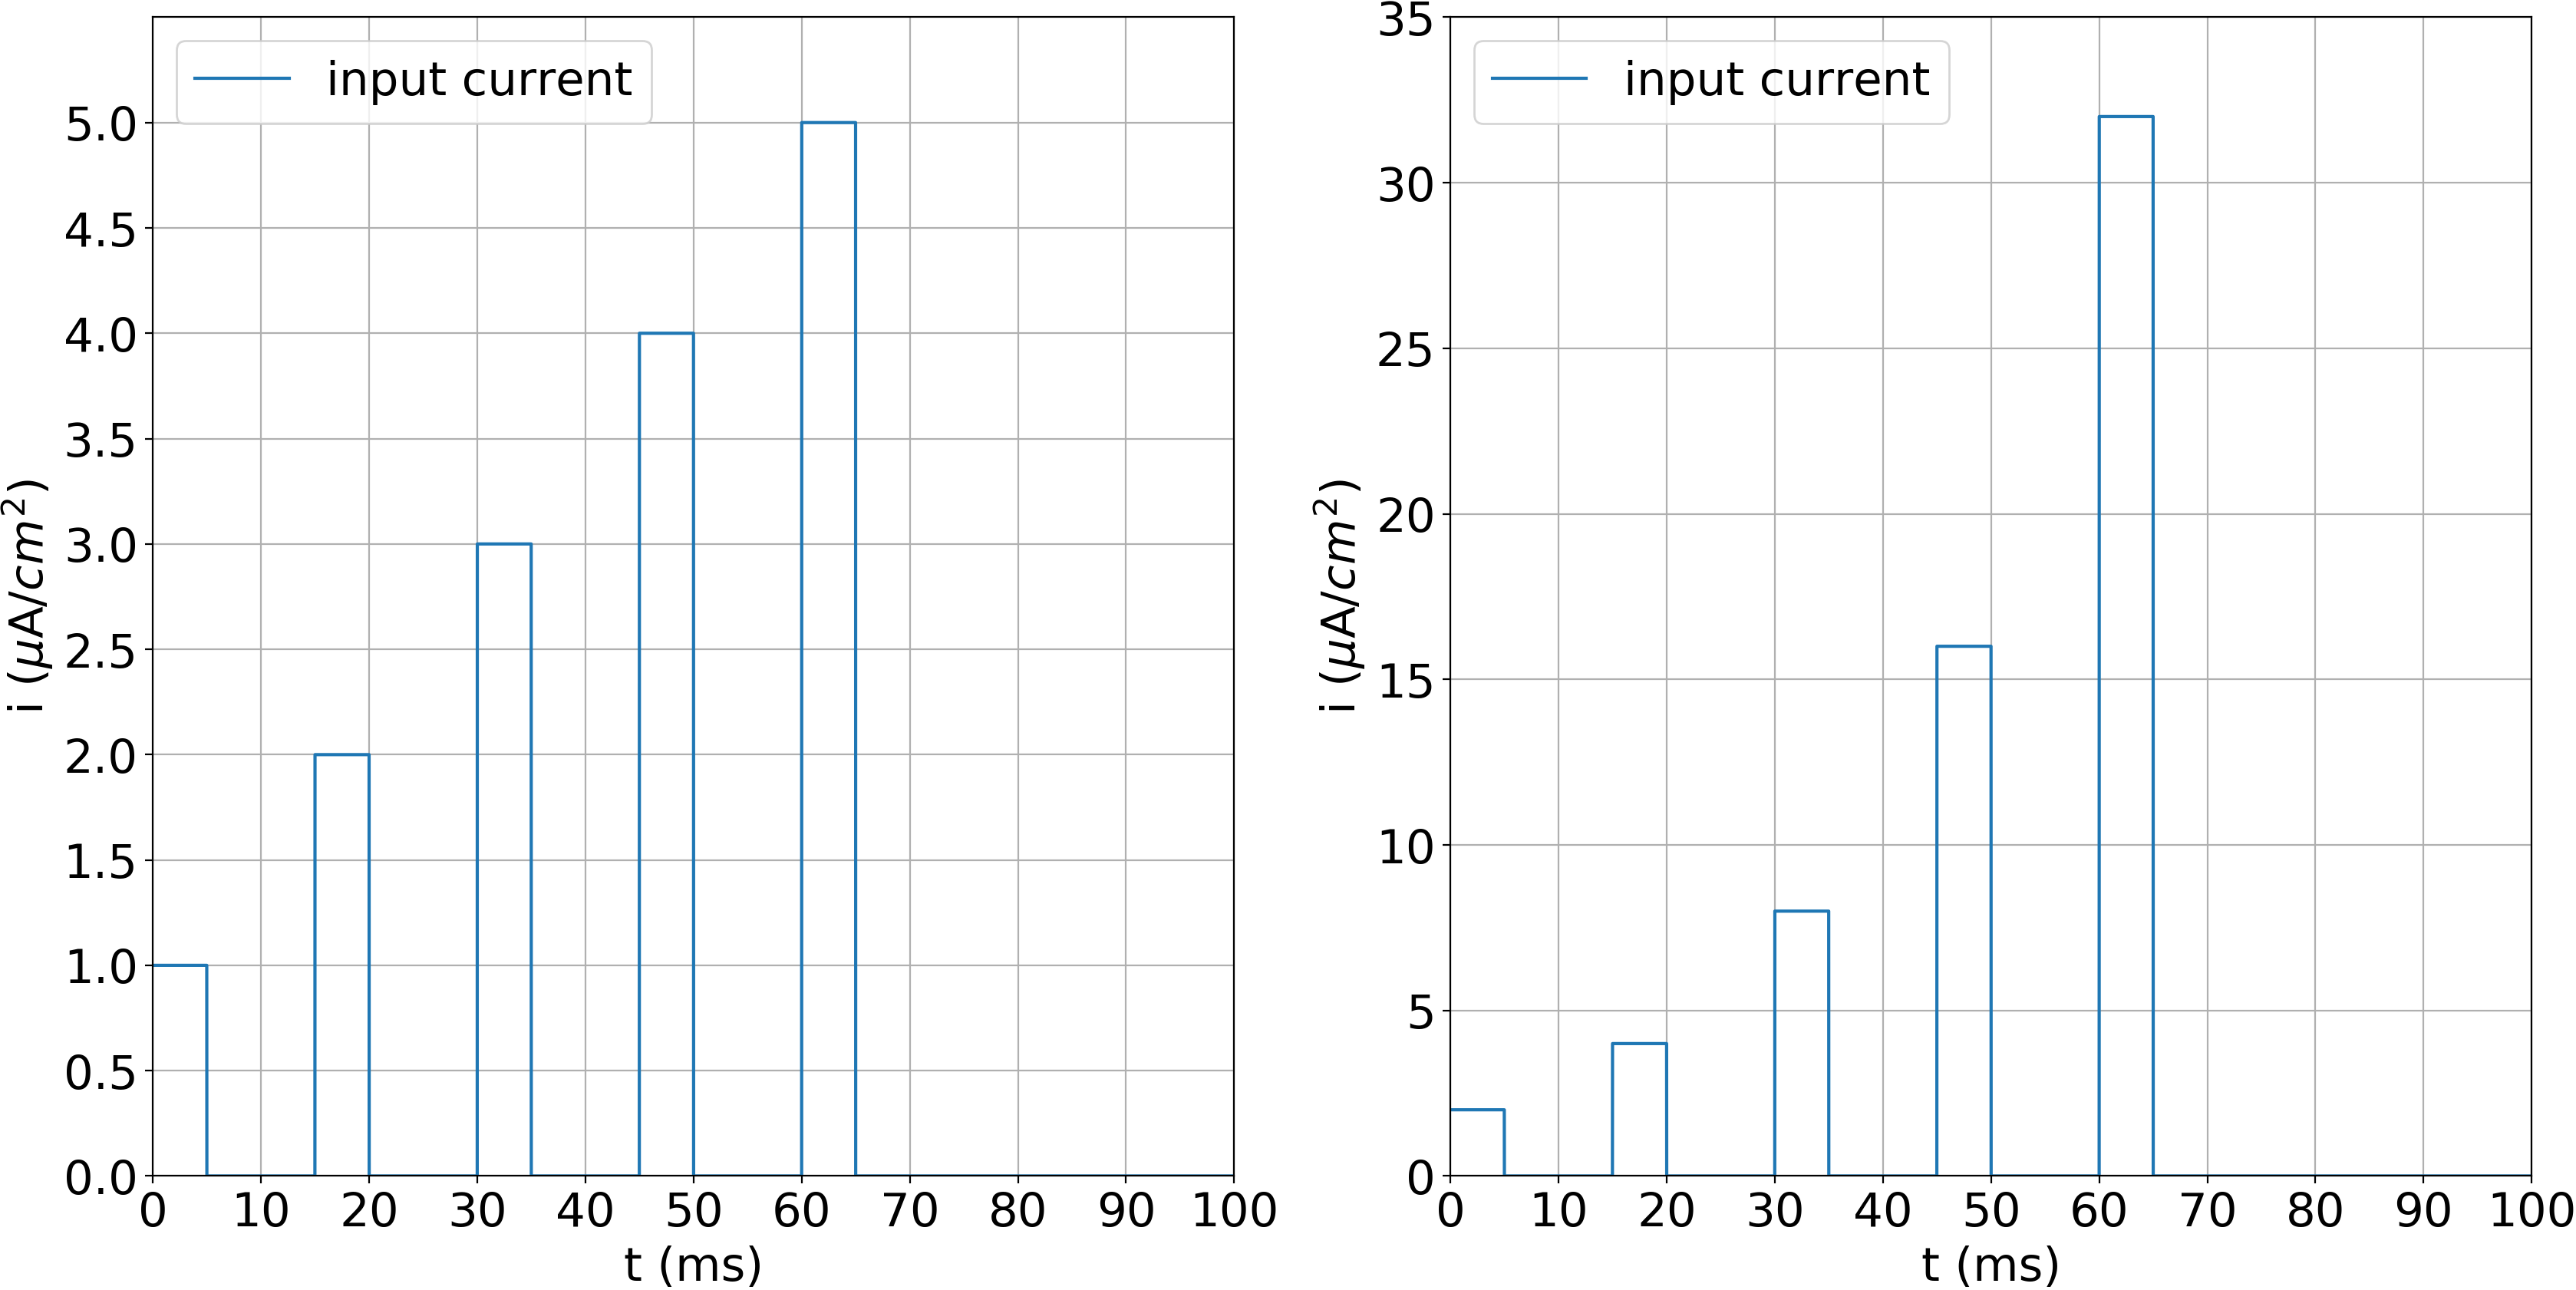
\includegraphics[scale=0.356]{2.png}
		\captionsetup{width=\linewidth}  %choose the with of the caption
		\caption{Input current densities for different temperatures.}
		\label{fig2} %choose a label, see subsection references
	\end{flushleft}
\end{figure}

\newpage
\subsection{Plots of experimental results 2.1}

\begin{figure}[hbpt!]					%start figure-environment
	\begin{flushleft}
		\hspace*{-0.1in}
		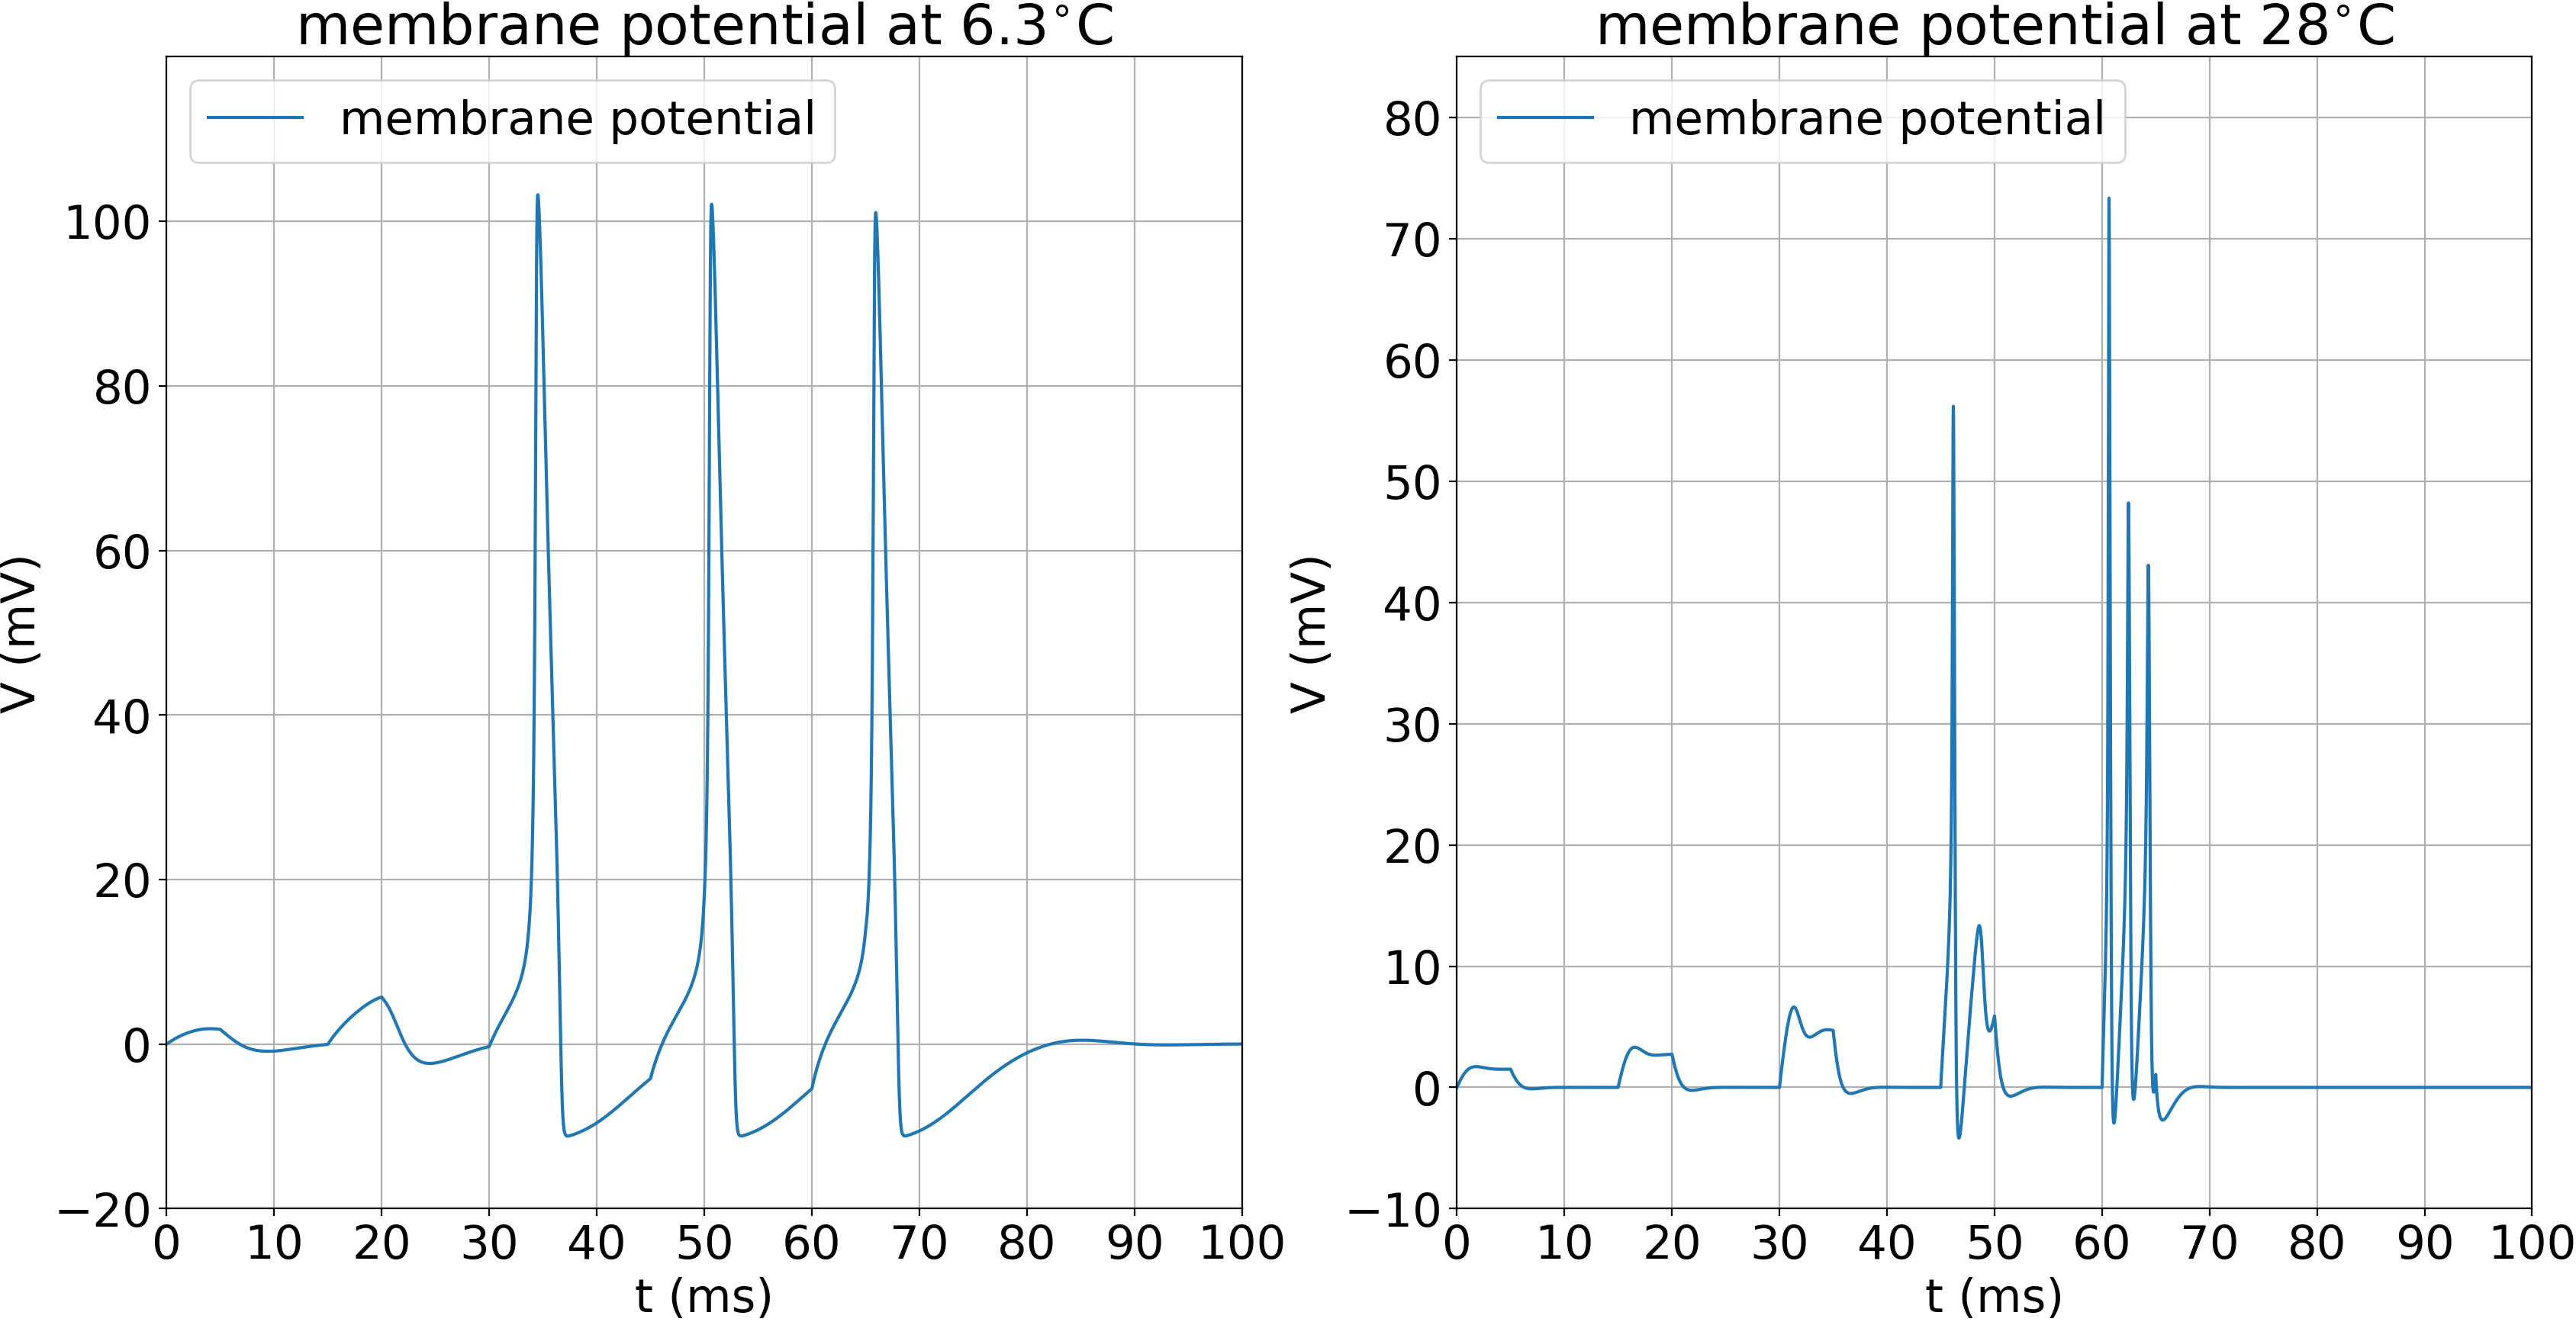
\includegraphics[scale=0.36]{3.png}
		\captionsetup{width=\linewidth}  %choose the with of the caption
		\caption{Membrane Potentials for the different cases}
		\label{fig3} %choose a label, see subsection references
	\end{flushleft}
\end{figure}

\begin{figure}[hbpt!]					%start figure-environment
	\begin{flushleft}
		\hspace*{-0.1in}
		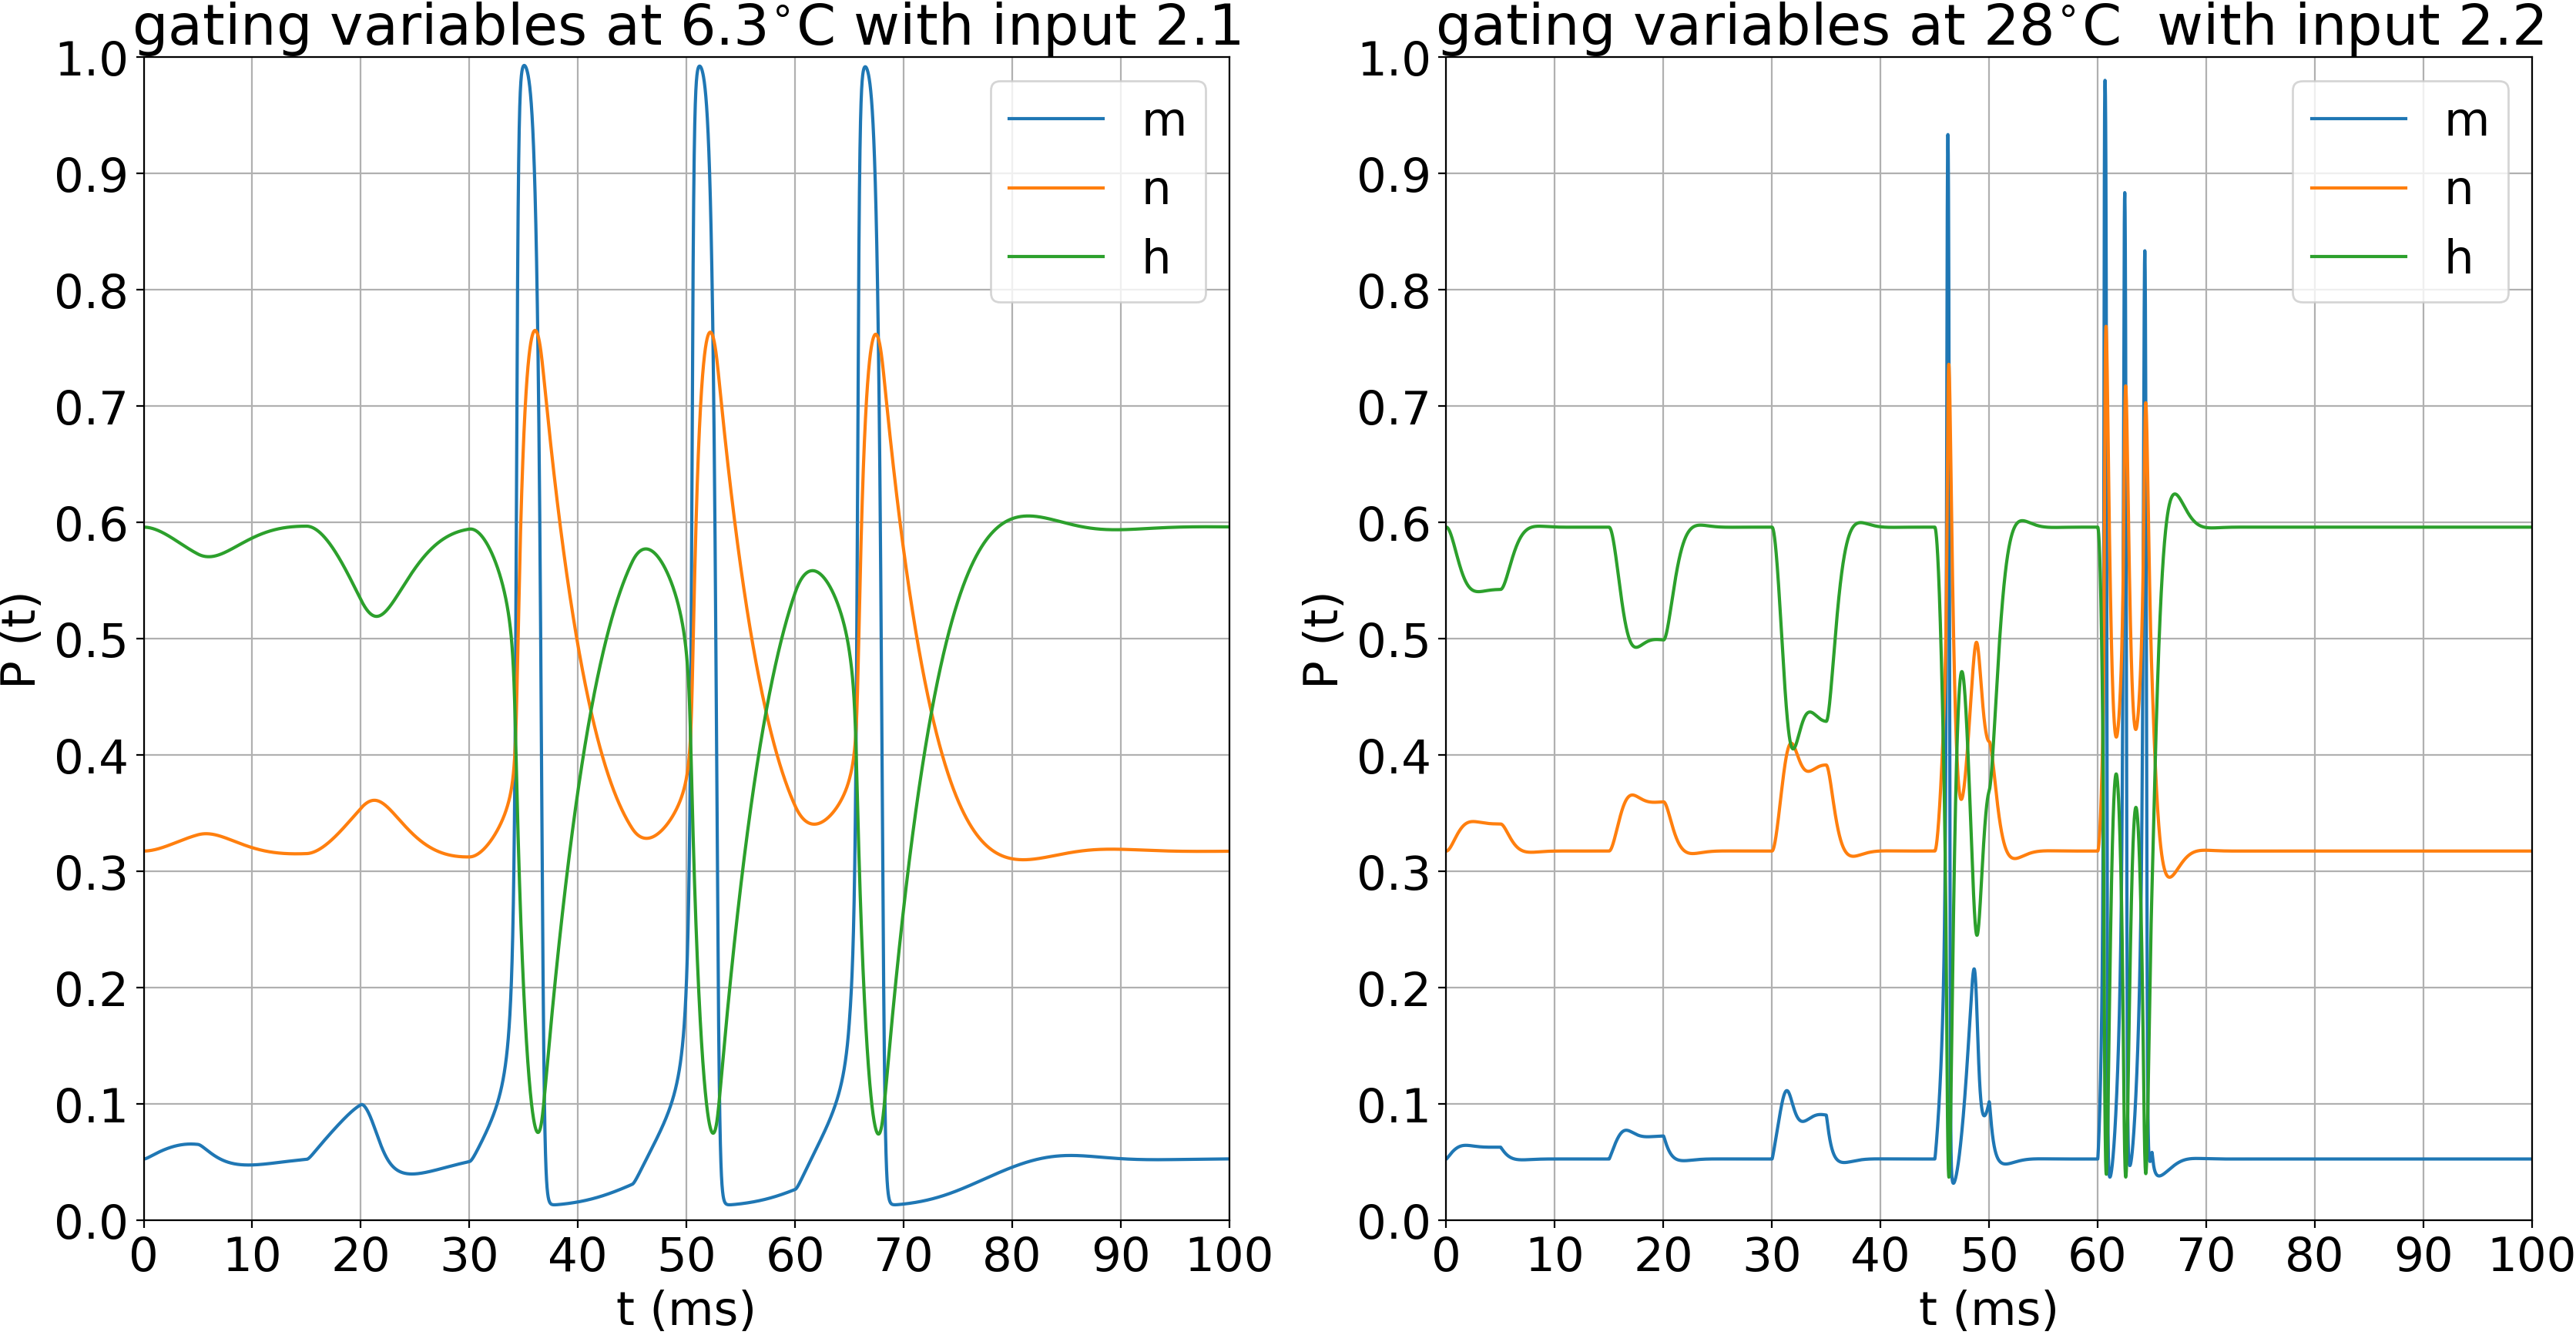
\includegraphics[scale=0.36]{4.png}
		\captionsetup{width=\linewidth}  %choose the with of the caption
		\caption{Gating Variables m, n, h for the different cases.}
		\label{fig3} %choose a label, see subsection references
	\end{flushleft}
\end{figure}

\newpage
\begin{figure}[hbpt!]					%start figure-environment
	\begin{flushleft}
		\hspace*{-0.1in}
			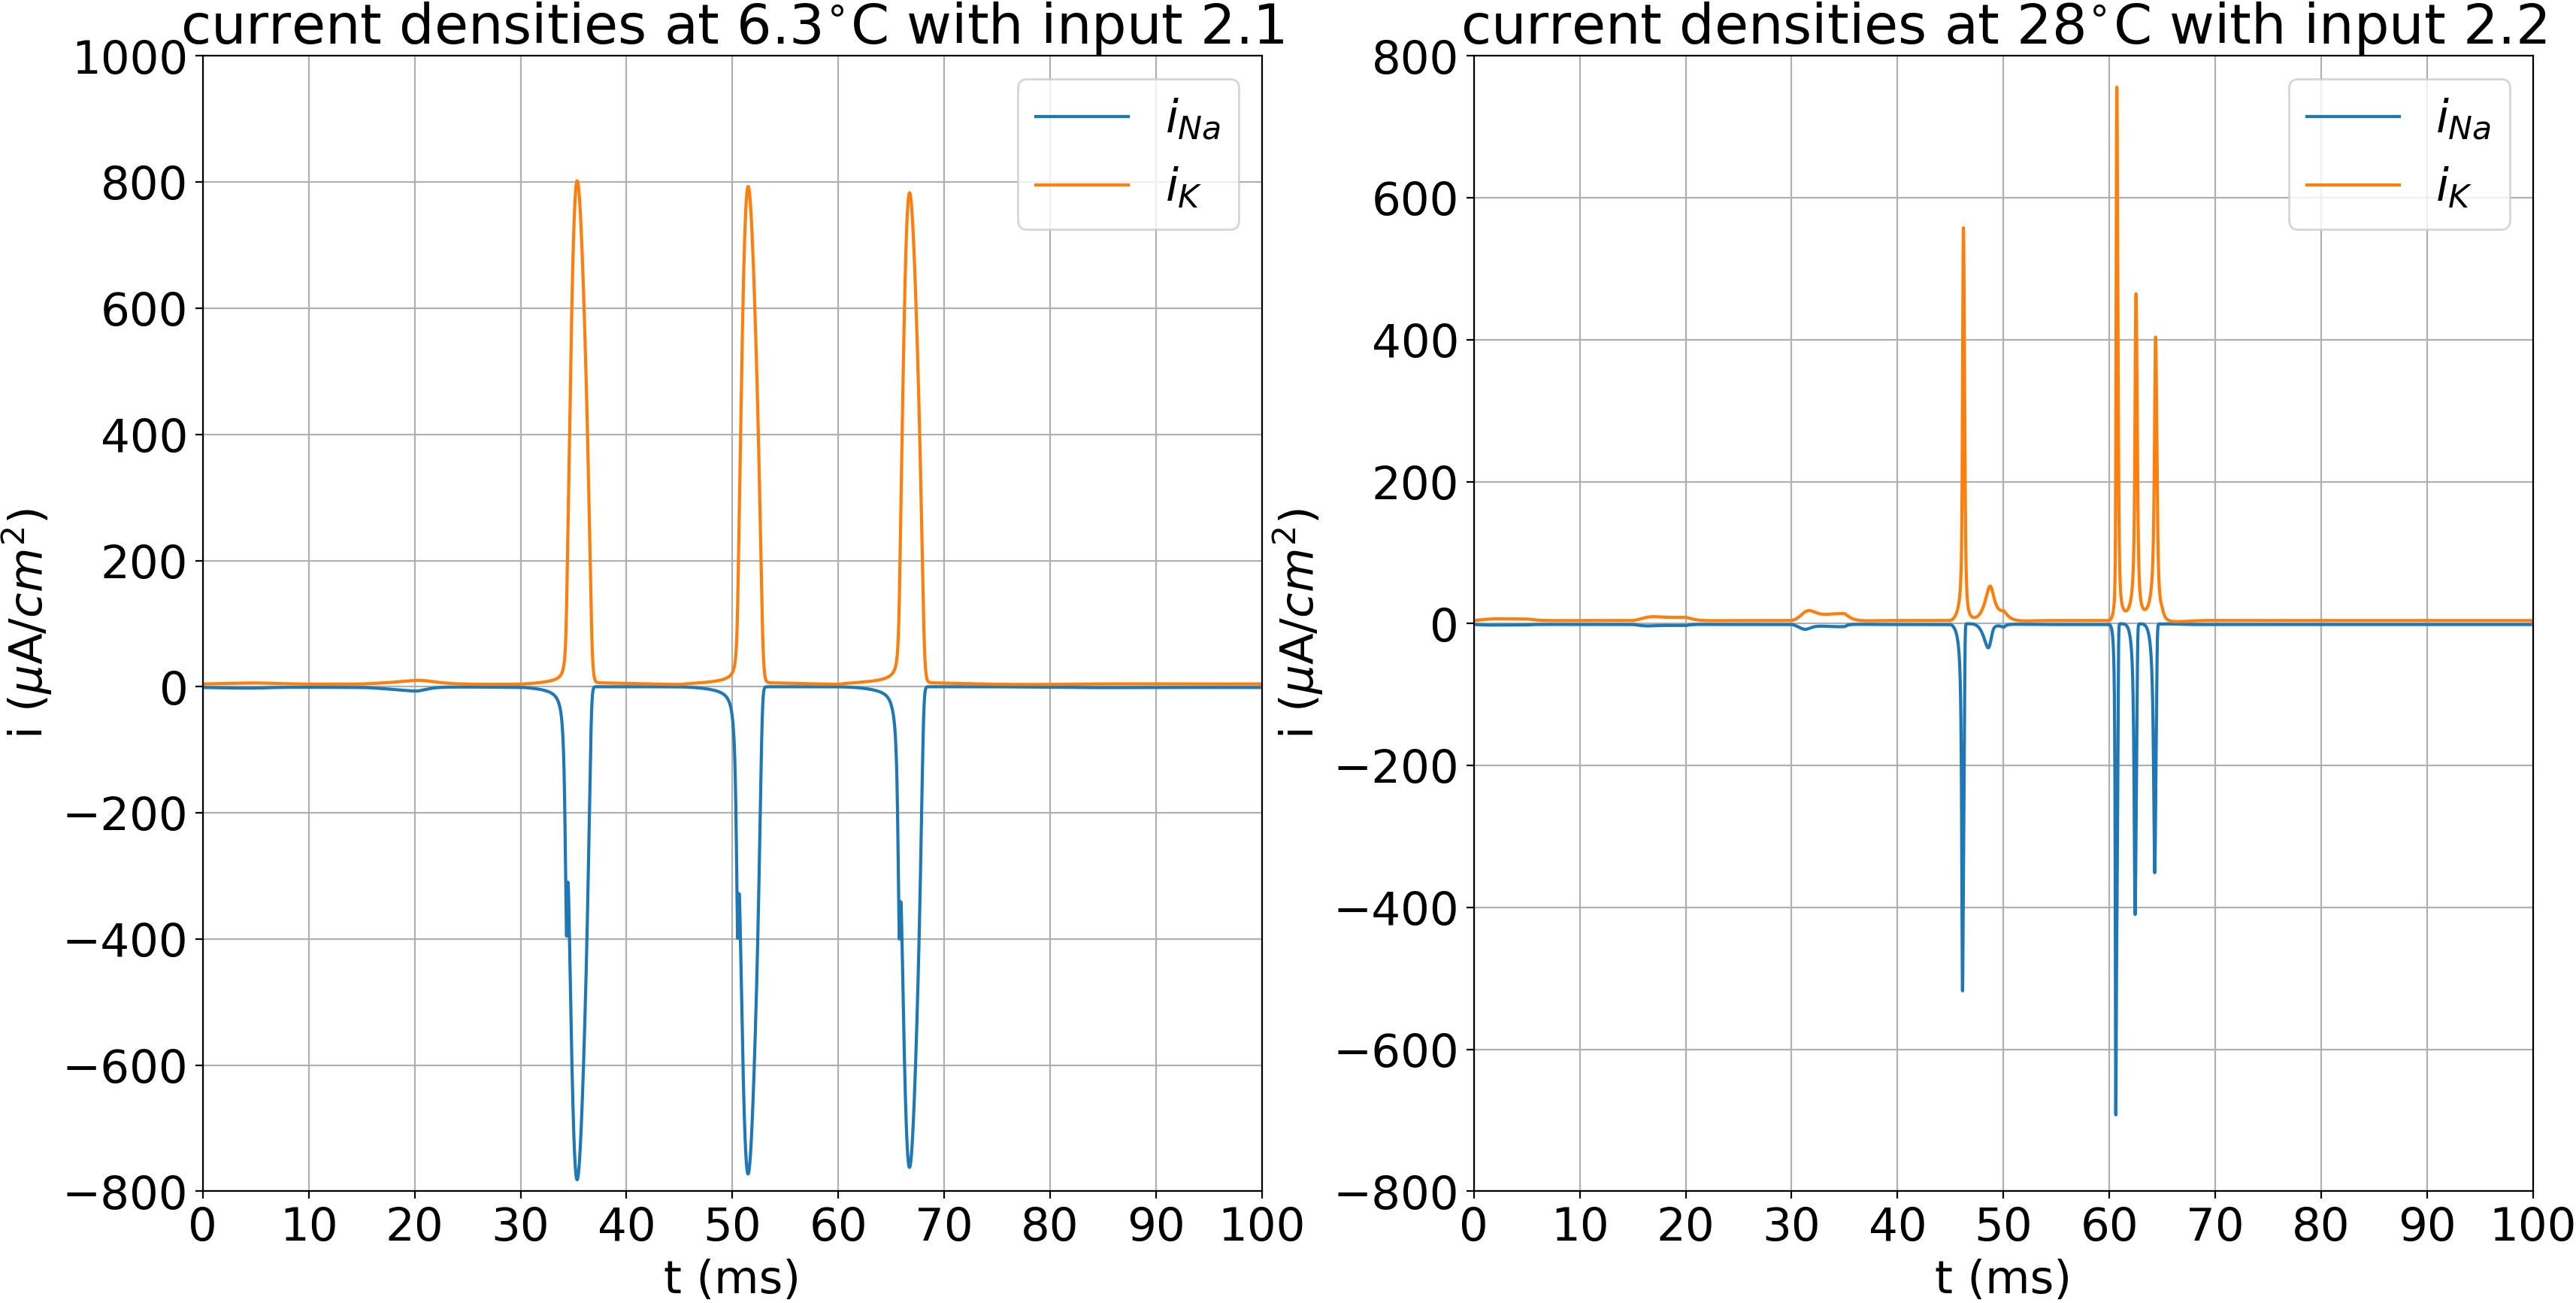
\includegraphics[scale=0.36]{5.png}
		\captionsetup{width=\linewidth}  %choose the with of the caption
		\caption{Current densities $i_{Na}$ and ${i_K}$ for the different cases}
		\label{fig5} %choose a label, see subsection references
	\end{flushleft}
\end{figure}

\begin{figure}[hbpt!]					%start figure-environment
	\begin{flushleft}
		\hspace*{-0.1in}
		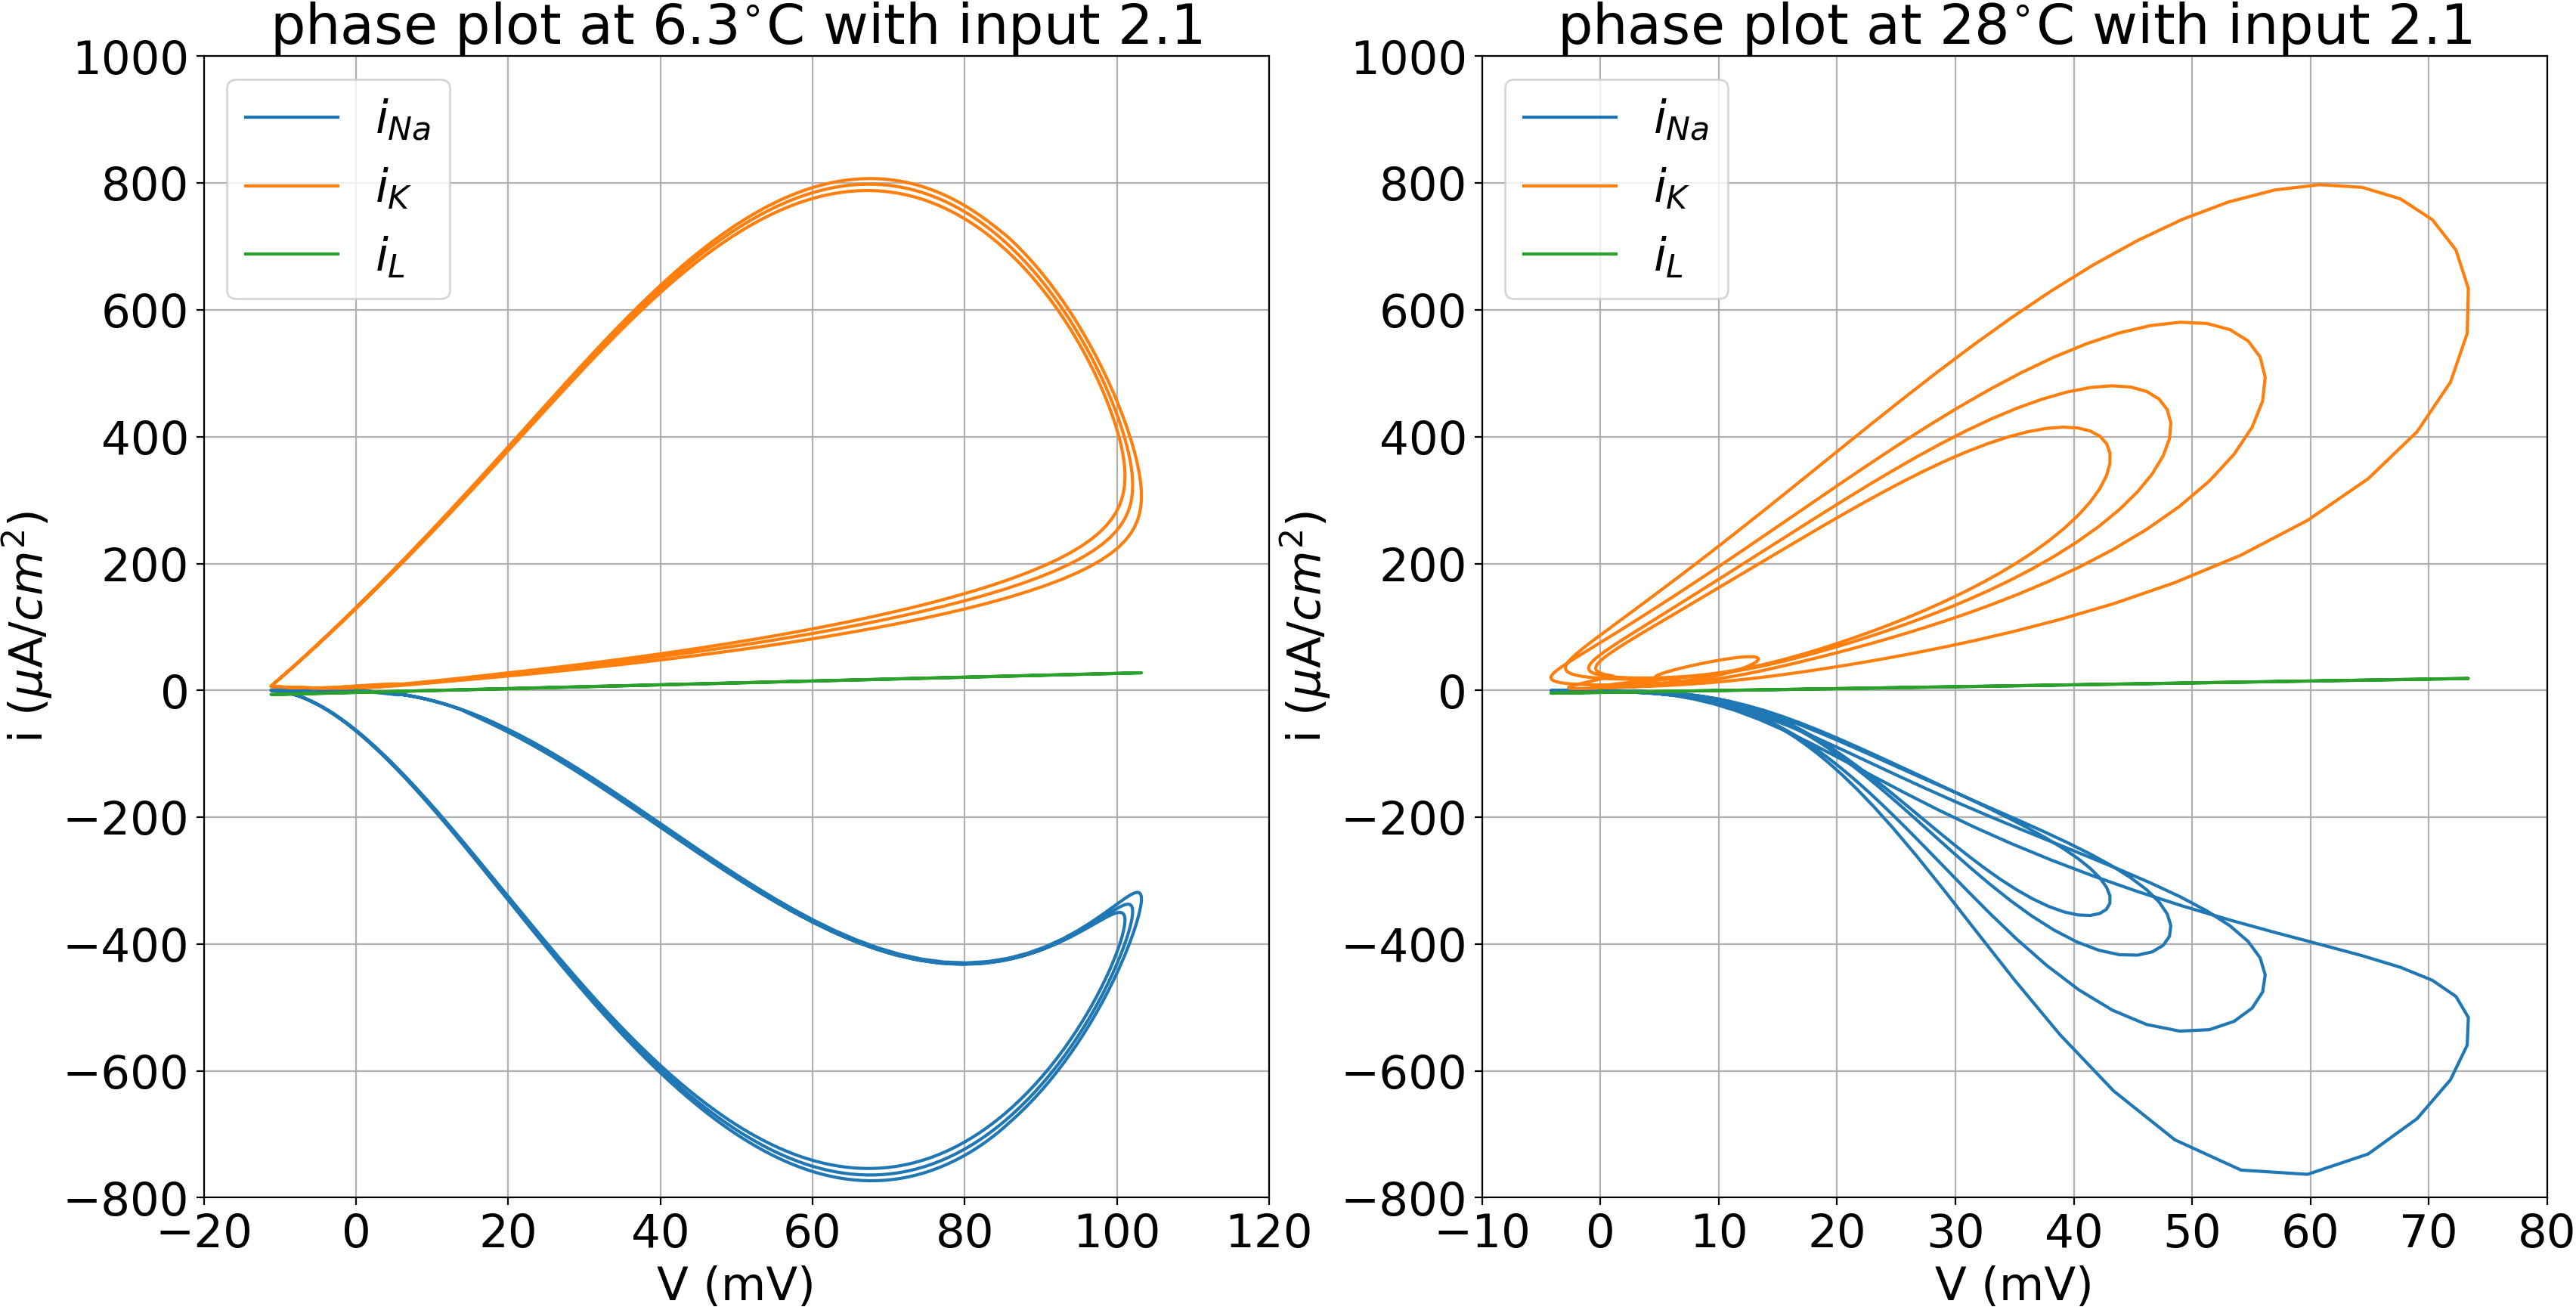
\includegraphics[scale=0.36]{6.png}
		\captionsetup{width=\linewidth}  %choose the with of the caption
		\caption{Phase plot for different cases.}
		\label{fig6} %choose a label, see subsection references
	\end{flushleft}
\end{figure}

\end{document}
